\chapter{基本原理介绍}
\section{正交频分复用技术的基本原理及分析}
\subsection{正交频分复用技术的基本原理}
\subsection{正交频分复用技术的特点分析}

\section{正交频分复用技术的关键技术}
\section{卷积码的基本概念}
卷积码与分组码不同,其编码器具有记忆性,即编码器的当前输出不仅与当前输入有关,还跟以前时刻的输入有关。分组码在编码时,先是将输入信息码元序列分为长度为k的段,然后按照编码规则,给每段附加上r位的监督码元,构成长度为n的码组。各个码组间没有约束关系,即监督码元之监督本码组的码元信息有无错误。因此,在解码时各个接收码组间也是独立地进行解码的,不能利用组间信息,且编码定理表明分组码的码长n越长越好,另一方面译码运算量却随着码长n的增加而增加。为解决这一问题,卷积码被提出。卷积码的特点是信息进行编码时,信息组之间不是独立编码的,而是具有一定的相关性。系统译码时可以利用这种相关性进行译码。卷积码一般表述成$(n,k,m)$的形式,码率为$R=k/n$。存储器阶数为$m$的卷积编码器可用$k$个输入、$n$个输出、输入存储器阶数为m的线性序贯电路实现,即输入在进入编码器后仍会多呆$m$个时间单元。通常,$n$和$k$都是比较小的整数,$k<n$,信息序列被分成长度为$k$的分组,码字(codeword)被分成长度为 $n$的分组。当 $k=1$时,信息序列无需分组,处理连续进行。值得注意的是,卷积码不像分组码,较大的最小距离和低错误概率不是通过增加$k$和$n$实现的,而是通过增加存储器阶数$m$实现的,即卷积码的纠错能力随着$m$的增大而增大,而复杂度随着m的增加而指数增加。在编码器复杂度相同的情况下,卷积码的性能要优于分组码的。

卷积码是1955年由 Elias(1923~2001)首次提出的,随后Wozencraft和Reiffen提出了序贯译码方法(对具有较大约束长度的卷积码非常有效)。1963 年,Massey 提出了一个效率不高、但易于实现的译码方法――门限译码,这使得卷积码大量应用于卫星和无线信道的数字传输中。1967 年,Viterbi 提出了最大似然(ML, Maximum Likelihood)译码算法,易于实现具有较小约束长度的卷积码的软判决译码。Viterbi 算法配合序贯译码的软判决,使卷积码在20 世纪 70 年代广泛应用在深空和卫星通信系统。1974 年,Bahl, Cocke, Jelinek 以及 Raviv(BCJR)针对具有不等先验概率信息比特的卷积码,提出了最大后验概率(MAP maximum a posteriori probability)译码算法。BCJR 算法近年来广泛应用到软判决迭代译码方案中,其中信息比特的先验概率在每次迭代时都发生变化。这两种算法的最优化目标略有不同:在 MAP 译码算法中,信息比特错误概率是最小的,而在 ML 译码算法中,码字错误概率是最小的,但两种译码算法的性能在本质上是相同的。由于 Viterbi 算法实现更简单,因此在实际应用比较广泛,但在迭代译码应用中,例如逼近 Shannon 限的 Turbo 码,常使用 BCJR 算法。另外,在迭代译码应用中,还有一种 Viterbi 算法的变种:软输出 Viterbi 算法(SOVA,Soft-Output Viterbi Algorithm),它是 Hagenauer 和 Hoeher 在 1989 年提出的。对卷积码描述最详尽的书籍是:
R. Johannesson and K.S. Zigangirov, Fundamentals of Convolutional Coding. IEEE Press, Piscataway , N. J., 1999.

\section{卷积编码原理及其描述方法}
\subsection{卷积码编码原理}
下面以$(2,1,2)$卷积码为例,简单说明卷积码的编码过程。
\begin{figure}[htbp]
	\centering
	\tikzset{%
		block/.style    = {draw, thick, rectangle, minimum height = 2em,
			minimum width = 3em},
		sum/.style      = {draw, circle, inner sep=0pt, node distance = 2cm}, % Adder
		input/.style    = {coordinate}, % Input
		output/.style   = {coordinate} % Output
	}
	\begin{tikzpicture}[auto, thick, node distance=2cm, >=stealth']
	\draw
	node [input] (in) {}
	node [block,right of=in] (d1) {$D_1$}
	node [block,right of=d1, node distance=3cm] (d2) {$D_2$}
	node [sum,above of=d1,xshift=1.5cm] (sum1) {\Large $+$}
	node [sum,below of=d1,xshift=1.5cm] (sum2) {\Large $+$}
	;
	
	\draw [->] (in) --node [below left] {$u_i$} (d1);
	\draw [->] (d1) --node [anchor=north] {$u_{i-1}$} (d2);
	\draw [->] (0.6,0) |- (sum1);
	\draw [->] (0.6,0) |- (sum2);
	\draw node[yshift=-0.04cm] at (0.6,0) {\textbullet};
	\draw node[yshift=-0.04cm] at (3.5,0){\textbullet};
	\draw [->] (3.5,0) -- (sum1);
	\draw  (d2) -- node[anchor=north] {$u_{i-2}$} +(1.5cm,0) node[yshift=-0.04cm](n1) {\textbullet};
	\draw [->,below of=0cm] (d2) ++(1.5cm,0) |- (sum1);
	\draw [->,below of=0cm] (d2) ++(1.5cm,0) |- (sum2);
	
	\draw (n1) ++(1.5cm,-0.04cm) node (rn1) {\textbullet};
	\draw (rn1) ++(-1.0cm,1.0cm) node[name=rn2]  {\Large \textopenbullet} node[above right] {$c_i^{(1)}$};
	\draw (rn1) ++(-1.0cm,-1.0cm) node {\Large \textopenbullet} node[below right] {$c_i^{(2)}$}++(0,-1.5cm);
	
	\draw [->] (n1)++(1.5cm,0) --+(-0.95cm,0.95cm);
	\draw [thin](n1)++(1.5cm,0)++(-1.0cm,1.06cm) --+(0,1.5cm) -| (sum1);
	\draw [thin] (n1)++(1.5cm,0)++(-1.0cm,-1.04cm)--+(0,-1.5cm) -| (sum2);
	
	\draw [->](n1) (n1)++(1.5cm,0) --+(1.5cm,0) node[output] {} node [above left] {$C$};
	\draw [<->,dashed](n1)++(1.5cm,0)++(0,0.8cm) arc (90:180:0.8);
	\end{tikzpicture}
	\caption{$(2,1,2)$卷积编码器}
\end{figure}

此电路由二级移位寄存器$D_1$、$D_2$、两个模2加法器及开关电路组成。编码前,各寄存器清零,信息码元按$u_1,u_2,u_3,\cdots,u_{i-1},u_{i},\cdots$的顺序输入编码器。每输入一个信息码元$u_i$ ,开关依次打到$c_i^{(1)}$、$c_i^{(2)}$端点各一次,输出一个子码$c_i^{(1)}c_i^{(2)}$。子码中的两个码元与输入信息码元之间的关系是:
\begin{equation}
\begin{split}
c_i^{(1)}&=u_i\oplus u_{i-1} \oplus u_{i-2} \\
c_i^{(2)}&=u_i\oplus u_{i-2}
\end{split}
\end{equation}

由此可见,第$i$个子码中的两个码元不仅与本子码信息码元$u_i$有关,而且还与前面两个子码中的信息码元$u_{i-1}$和$u_{i-2}$有关,该卷积码的编码存储$u=2$,约束长度$N=u+1=3$。

\subsection{卷积码的描述方式}
描述卷积码的方法有很多,大致可以分为两大类:解析法和图形法。卷积码可以分别用码的多项式、矩阵生成法、离散卷积法、状态图、码状图和网格图等来描述。前三种属于数学描述,后面的三种属于卷积码的图形描述。下面将以图一为例着重讲述卷积码的生成多项式法和网格图。

如图\ref{figure:theory:pic2}所示,我们将卷积编码器表示成如下图形:
\begin{figure}[htbp]
	\centering
	\tikzset{%
		block/.style    = {draw, thick, rectangle, minimum height = 10em,
			minimum width = 3em},
		sum/.style      = {draw, circle, inner sep=0pt, node distance = 2cm}, % Adder
		input/.style    = {coordinate}, % Input
		output/.style   = {coordinate} % Output
	}
	\begin{tikzpicture}[auto, thick, node distance=2cm, >=stealth']
	\draw
	node [input] (in) {}
	node [block, right of=in,text width =2em,node distance = 9em] (b1) {串/并转换}
	node [block, right of=b1,text width =2em,node distance = 3cm] (b2) {有限状态的有记忆系统}
	node [block, right of=b2,text width =2em,node distance = 3cm] (b3) {并/串转换}
	node [output, right of=b3,node distance = 9em] (out) {};
	;
	
	\draw [->] (in)--node[above] {输入信息序列}(b1);
	\draw [->] (b3)--node [above] {输出信息序列}(out);
	\draw [->] (b1)++(1.5em,1.5cm) -- node[anchor=south] {$u_1$} ++(3cm-3em,0);
	\draw [->] (b1)++(1.5em,1.0cm) -- node[anchor=south] {$u_2$} ++(3cm-3em,0);
	\draw [->] (b1)++(1.5em,-1.5cm) -- node[anchor=south] {$u_1$} ++(3cm-3em,0);
	\draw node[text width =1em,right of=b1,node distance=1.5cm-0.5em] {$\textbullet$~$\textbullet$~$\textbullet$};
	\draw [->] (b2)++(1.5em,1.5cm) -- node[anchor=south] {$c_1$} ++(3cm-3em,0);
	\draw [->] (b2)++(1.5em,1.0cm) -- node[anchor=south] {$c_2$} ++(3cm-3em,0);
	\draw [->] (b2)++(1.5em,-1.5cm) -- node[anchor=south] {$c_1$} ++(3cm-3em,0);
	\draw node[text width =1em,right of=b2,node distance=1.5cm-0.5em] {$\textbullet$~$\textbullet$~$\textbullet$};
	
	
	\end{tikzpicture}
	\caption{卷积编码器原理图}
	\label{figure:theory:pic2}
\end{figure}

编码器的输入是由$k$个信息元组成的信息组$u_i$,那么相应的输出则是由$n$个$c_i$组成的序列若输入是一个半无限序列,则由卷积码编码器输出的序列也是一个半无限序列,此序列称为卷积码的一个码序列或者码字。我们可以将输入的序列写成多项式的形式。

若$\bm{u}=(u_1u_2u_3u_4u_5\cdots)$,则
\[
u(x)=u_0+u_1x+u_2x^2+\cdots
\]
所以
\[
\bm{u}=(101)\to u(x)=1+x^2
\]
在以下分析中,我们定义系数
\begin{equation}
\begin{split}
\bm{g}_k^1=(g_{k,0}^1g_{k,1}^1 & g_{k,2}^1\cdots g_{k,m}^1) \\
\bm{g}_k^2=(g_{k,0}^2g_{k,1}^2 & g_{k,2}^2\cdots g_{k,m}^2) \\
&\vdots \\
\bm{g}_k^n=(g_{k,0}^ng_{k,1}^n & g_{k,2}^n\cdots g_{k,m}^n) \\
\end{split}
\end{equation}


它们用来表示第$k$个输入端在输出端$c^1,c^2,\cdots,c^n$的求和系数,由于图一中的$k=1$,故在下面的分析中省略角标$k$,则有
\begin{equation}
\bm{g}^1=(111),\bm{g}^2=(101)
\end{equation}
那么对应多项式为
\begin{equation}
g^1=1+x+x^2,g^2=1+x^2
\end{equation}
编码后的多项式(相乘之后模二加)
\begin{equation}
\begin{cases}
c^1=u(x)\cdot g^1(x) \\
c^2=u(x) \cdot g^2(x)
\end{cases}
\end{equation}
最后得到
\begin{equation}
\begin{cases}
c^1=u(x)\cdot g^1(x) = (1+x^2)(1+x+x^2)=1+x+x^3+x^4 \\
c^2=u(x) \cdot g^2(x) = (1+x^2)(1+x^2)=1+x^4
\end{cases}
\end{equation}

\subsubsection{卷积码编码图形描述}
i)状态图

在卷积编码器中,寄存器任一时刻存储的数据称为编码器的一个状态,随着信息序列的不断输入,编码器的状态在不断变化,同时输出的码元序列也随之改变。所谓状态图就是反应编码器中寄存器存储状态转移的关系图,它用编码器中寄存器的状态及其随着输入序列而发生的转移关系来描述编码过程的。如图\ref{figure:theoty:pic3}所示:
\begin{figure}[htbp]
	\centering
	\tikzset{%
		block/.style    = {draw, thick, rectangle, minimum height = 10em,
			minimum width = 3em},
		sum/.style      = {draw, circle, inner sep=1pt, node distance = 2cm}, % Adder
		input/.style    = {coordinate}, % Input
		to/.style={->,>=stealth',shorten >=1pt,semithick,font=\sffamily\footnotesize},
		output/.style   = {coordinate} % Output
	}
	\begin{tikzpicture}[auto, thick, node distance=4cm,->,>=stealth']
	\draw
	node [sum,name=n00] at (0,0) {00}
	node [sum,name=n01] at (2cm,-2cm) {01}
	node [sum,name=n10] at (2cm,2cm) {10}
	node [sum,name=n11] at (4cm,0) {11};
	\path
	(n00) edge[very thin,bend left=20,dashed] node[anchor=north,above]{11} (n10)
	(n00) edge[thin,loop left]    node[anchor=north,above]{00} (n00)
	(n10) edge[thin,bend left=20,dashed] node[anchor=north,above]{01} (n11)
	(n11) edge[thin,loop right] node[anchor=north,above]{10} (n11)
	(n11) edge[thin,bend left=20] node[anchor=north,below]{01} (n01)
	(n01) edge[thin,bend left=20] node[anchor=north,below]{11} (n00)
	(n01) edge[thin,bend left=10] node [anchor=east] {00} (n10)
	(n10) edge[thin,bend left=10,dashed] node[anchor=west]{10} (n01);
	
	
	\end{tikzpicture}
	\caption{卷积码状态图}
	\label{figure:theoty:pic3}
\end{figure}

图中圆圈中的数字表示寄存器的状态,共有四个不同的状态:00、01、10、11。连接圆圈之间的箭头方向表示状态转移的方向,若输入信息比特为1,连接的箭头用虚线表示;若为0,则用实线表示。连线旁的两位数字表示相应的输出子码。箭头所指的状态即为该信息码元移入编码器后的状态。

ii)码状图

码状图结构是由状态图按时间展开的。即将输入信息序列 的输入顺序按时间顺序展开并展开所有可能的输入输出情况。如果 卷积码编码器的输入信息序列是半无限长序列,则它输出的码元序列也是一个半无限长的序列,这种时候也就需要半无限长的码状图来描述。
\begin{figure}[htbp]
	\centering
		\def\refpath#1#2#3#4#5{--node[above,xshift=(#1)/8] {#3}++(-#1,0) -- node[right]{#4} ++(0,-#2) -- node[above,xshift=(#1)/8]{#5} ++(#1,0)}
		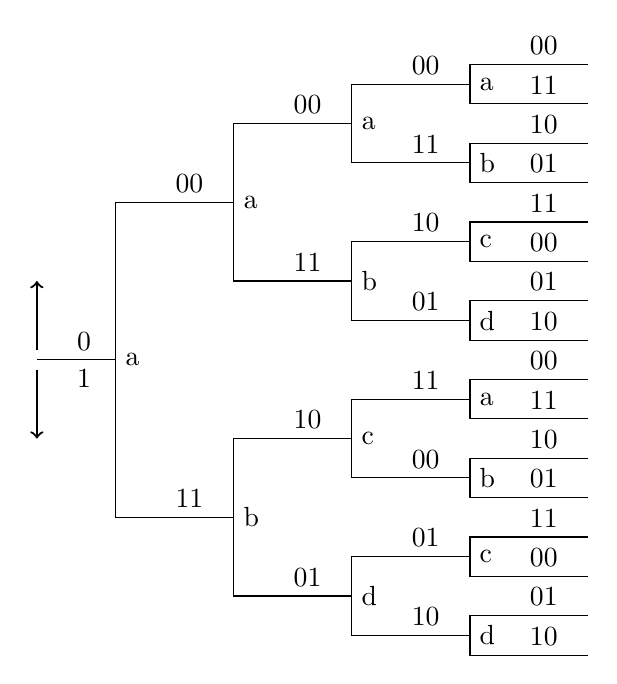
\begin{tikzpicture}
		%\draw node (in) {};
		\draw  (0,0) \refpath{1.5cm}{0.5cm}{\xiaowu 00}{\xiaowu a}{\xiaowu 11};
		\draw  (0,-1cm) \refpath{1.5cm}{0.5cm}{\xiaowu 10}{\xiaowu b}{\xiaowu 01};
		\draw  (0,-2cm) \refpath{1.5cm}{0.5cm}{\xiaowu 11}{\xiaowu c}{\xiaowu 00};
		\draw  (0,-3cm) \refpath{1.5cm}{0.5cm}{\xiaowu 01}{\xiaowu d}{\xiaowu 10};
		
		\draw  (0,-4cm) \refpath{1.5cm}{0.5cm}{\xiaowu 00}{\xiaowu a}{\xiaowu 11};
		\draw  (0,-5cm) \refpath{1.5cm}{0.5cm}{\xiaowu 10}{\xiaowu b}{\xiaowu 01};
		\draw  (0,-6cm) \refpath{1.5cm}{0.5cm}{\xiaowu 11}{\xiaowu c}{\xiaowu 00};
		\draw  (0,-7cm) \refpath{1.5cm}{0.5cm}{\xiaowu 01}{\xiaowu d}{\xiaowu 10};
		
		%% second row
		\draw  (-1.5cm,-0.25cm) \refpath{1.5cm}{1.0cm}{\xiaowu 00}{\xiaowu a}{\xiaowu 11};
		\draw  (-1.5cm,-2.25cm) \refpath{1.5cm}{1.0cm}{\xiaowu 10}{\xiaowu b}{\xiaowu 01};
		\draw  (-1.5cm,-4.25cm) \refpath{1.5cm}{1.0cm}{\xiaowu 11}{\xiaowu c}{\xiaowu 00};
		\draw  (-1.5cm,-6.25cm) \refpath{1.5cm}{1.0cm}{\xiaowu 01}{\xiaowu d}{\xiaowu 10};
		
		%% third
		\draw  (-3cm,-0.75cm) \refpath{1.5cm}{2.0cm}{\xiaowu 00}{\xiaowu a}{\xiaowu 11};
		\draw  (-3cm,-4.75cm) \refpath{1.5cm}{2.0cm}{\xiaowu 10}{\xiaowu b}{\xiaowu 01};
		
		%% fourth row
		\draw  (-4.5cm,-1.75cm) \refpath{1.5cm}{4.0cm}{\xiaowu 00}{\xiaowu a}{\xiaowu 11};
		
		\draw (-6cm,-3.75cm) -- node[above,xshift=0.1cm]{0} node[below,xshift=0.1cm]{1}++(-1cm,0) node (in) {};
		
		\draw [->,thick] (in) --+(0,1cm);
		\draw [->,thick] (in) --+(0,-1cm);
		
		\end{tikzpicture}
	\caption{卷积码的码状图}
	\label{figure:theory:pic4}
\end{figure}

在码状图中,编码的过程相当于以输入信息为指令沿着码树游走,在树图中所经过的路径代码则是相应的输出。码树图最大的特点是按时间顺序展开的,并且能将所有时间状态表示为不相重合的路径。一般地,对于二元$(n,k,m)$卷积码来说,从每个节点出发有$2^k$分支,每个分支上有长度为$n$的码输出,最多有$2^{km}$种可能。

我们可以从图中看到,状态图看上去最为简洁,但是时序关系不清晰,然而码状图的最大特点就是时序关系很清晰,但是进行到一定时序后状态产生重复,树图变得复杂起来。

iii)网格图

网格图又称篱笆图,他综合了状态图和码状图的特点,是将码状图中的处于同一级节点合并而成的,是一个纵深宽度或高为 $2^{km}$的网格图,结构简单,而且时序关系清晰。网格图的最大特点是保持了码状图的时序展开性,同时又克服了码状图中太复杂的特点,它将码状图中的重复状态合并起来。

从图\ref{figure:theory:pic4}中可以看到,从某一阶节点开始所长出的分支从纵向看是周期重复的。下面的图\ref{figure:theory:pic5}为信息序列$l=5$的$(2,1,2)$卷积码的网格图,实现表示输入是0的分支,虚线表示输入是1的分支。分支上标注的 位数据表示相应的编码器的输出 。
\begin{figure}[htbp]
	\centering
	\def \nod{~~~~}
	\def \zihao{\wuhao}
	\tikzstyle{neuron}=[circle,fill=black!25,minimum size=0pt,inner sep=0pt]
	\tikzstyle{num}=[circle,fill=red!25,minimum size=0pt,inner sep=0pt]
	\begin{tikzpicture}[->,>=stealth',node distance=1.5cm]
	% a=00 layer
	\draw 
	node[neuron](a1) {\nod}
	++(1.5,0)node[neuron](a2){\nod}
	++(1.5,0)node[neuron](a3){\nod}
	++(1.5,0)node[neuron](a4){\nod}
	++(1.5,0)node[neuron](a5){\nod}
	++(1.5,0)node[neuron](a6){\nod}
	++(1.5,0)node[neuron](a7){\nod}
	++(1.5,0)node[neuron](a8){\nod}
	;
	
	% b=10 layer
	\draw 
	node [neuron,below of=a2] (b2) {\nod} (b2)
	++(1.5,0)node[neuron](b3){\nod}
	++(1.5,0)node[neuron](b4){\nod}
	++(1.5,0)node[neuron](b5){\nod}
	++(1.5,0)node[neuron](b6){\nod}
	;
	
	% c=01 layer	
	\draw 
	node [neuron,below of=b3] (c3) {\nod} (c3)
	++(1.5,0)node[neuron](c4){\nod}
	++(1.5,0)node[neuron](c5){\nod}
	++(1.5,0)node[neuron](c6){\nod}
	++(1.5,0)node[neuron](c7){\nod}
	;
	% d=11 layer
	\draw 
	node [neuron,below of=c3] (d3) {\nod} (d3)
	++(1.5,0)node[neuron](d4){\nod}
	++(1.5,0)node[neuron](d5){\nod}
	++(1.5,0)node[neuron](d6){\nod}
	;
	
	% a->a
	\foreach \source/\dest in {1/2,2/3,3/4,4/5,5/6,6/7,7/8}
	\path (a\source) edge node[num,sloped] {\zihao 00} (a\dest);
	
	% a->b
	\foreach \src/\dst in {1/2,2/3,3/4,4/5,5/6}
	\path (a\src) edge[dashed] node[num,fill=blue!35,sloped,xshift=-0.4cm] {\zihao 11} (b\dst);
	
	% b->c
	\foreach \source/\dest in {2/3,3/4,4/5,5/6,6/7}
	\path (b\source) edge node[num,fill=green!35,sloped,xshift=0.4cm] {\zihao 10} (c\dest);
	
	% b->d
	\foreach \source/\dest in {2/3,3/4,4/5,5/6}
	\path (b\source) edge[dashed] node[num,fill=orange!35,sloped] {\zihao 01} (d\dest);
	
	% d->c
	\foreach \source/\dest in {3/4,4/5,5/6,6/7}
	\path (d\source) edge node[num,fill=red!75,sloped] {\zihao 01} (c\dest);
	
	% c->b
	\foreach \source/\dest in {3/4,4/5,5/6}
	\path (c\source) edge[dashed] node[num,fill=yellow!25,sloped,xshift=0.4cm] {\zihao 00} (b\dest);
	
	% c->a
	\foreach \source/\dest in {3/4,4/5,5/6,6/7,7/8}
	\path (c\source) edge node[num,fill=blue!45!red,sloped,xshift=0.3cm] {\zihao 00} (a\dest);
	
	%d->d
	\foreach \source/\dest in {3/4,4/5,5/6}
	\path (d\source) edge[dashed] node[num,fill=green!25!pink,sloped] {\zihao 01} (d\dest);
	
	\draw 
	node[left of=a1,node distance=1cm] (a)  {$a=00$} (a)
	node[below of=a] (b) {$b=10$}
	node[below of=b] (c) {$c=01$}
	node[below of=c] (d) {$d=11$};
	;
	\draw node at (0,1) {};
	
	\end{tikzpicture}
	\caption{卷积码的网格图}
	\label{figure:theory:pic5}
\end{figure}


从第$m$至$l$节点,编码器处于稳定的状态转移中,并且各节点的网格结构均相同。在$l$节点后$m$个移位寄存器仍需转移$m$个状态,才能回到初始状态$a$。与码状图一样,网格图中每一种信息序列有唯一的网格编码路径。

\section{卷积码的译码}
卷积码的译码大致可以分为两大类:一类是代数译码,另一类则是概率译码。其中概率译码实际上就是常采用的卷积译码方式,它不仅基于码的代数结构,而且还利用了信道的统计特性,因此他充分地发挥了卷积码的特点,使得译码概率达到最小。对于长度为$l$的二进制码序列的最佳译码,如果用概率译码,需要对可能发送的$2l$个不同序列(即$2l$条可能路径)的对数似然函数累加值(即路径度量)进行比较,选择其中大路径度量即最小汉明距离的一条作译码结果。显然,译码过程的计算量随$l$增加而指数增长,这在实际中难以实现,因此只能采用次最佳的译码方法,其中之一是维特比(Viterbi)译码,根据判决的电平不同,又可以分为软判决和硬判决。
\subsection{硬判决的维特比译码}
维特比译码是一种最大似然译码。其基本思想是:将已经接收到的码字序列与所有可能的发送序列进行比较,选择其中码距最小的一个序列作为发送序列(即译码后的输出序列)。这个算法在实际应用中是采用迭代方式来处理的。在每一步中,它将进入每一状态的所有路径的度量值进行比较,并存储具有最大度量值的路径,即幸存路径。其具体步骤可归纳如下:

(1) 从起始状态( )开始到 时刻,计算进入每一状态的单个路径的部分度量值,并存储每一状态下的幸存路径及其度量值。
(2)从 到 共有 (状态数 个,每个状态下有 条路径)路径,计算每个分支上的码字与相应时间段内接收码字间的码距,分别与前面保留路径的码距相加,对到达 时刻的各状态的路径进行比较,每个状态保留一条最小码距的路径及相应的码距值,并删去所有其他路径。
(3) 按照步骤二进行下去,直到比较完所有的接收码字。
(4) 所有的码字比较完毕后,剩下 条路径(每个状态剩下一个路径),选择最小码距的路径,此路径上的发送码字序列即是译码后的输出序列。

上述三个步骤中,第一步是第二步的初始化,第三步是第三步的继续,所以关键在第二步。它主要包括两部分:一是对每个状态进行关于度量的计算和比较,从而决定幸存路径;另一个是对每一状态记录幸存路径及其度量值。其中两部分的第一部分,实质上是对网格图中间结点作局部优化判决,由于路径具有可分离性,即每条路径的度量值可写成组成它的各条分支的度量和,因此它满足动态规划的最优化原理,即这些局部优化运算等效于整体最优化。由此可知,在篱笆图上用维特比译码算法得到的路径一定是一条最大似然路径,因而这种译码方法是最佳的。Viterbi译码具有以下特点:
\begin{publist}
	\item 有利于译码器的硬件实现,运行速度快
	\item 译码时间固定
	\item 译码的错误概率可以达到很小
	\item 容易实现且成本很低。
\end{publist}

\subsection{软判决的维特比译码}
上面是硬判决译码,为了充分利用信息输出信号所提供的有关信息,提高译码性能,可以不将解调器输出波形进行硬判决成${0,1}$,而是进行多电平量化,然后再输入维特比译码器,称这种适应$Q$进制输入的维特比译码器为软判决维特比译码器。和硬判决译码器一样,软判决维特比译码器就是寻找与接收序列$R$有最小软判决距离的路径。因此,如果用最小软判决距离代替汉明距离作为选择幸存路径和译码器输出的准则,则软判决维特比译码器的结构和译码过程,完全与硬判决的相同,只要在$R$与$C$中用$Q$进制值即可,这里不再重复。
\section{卷积码的性能仿真分析}
下面通过MATLAB对OFDM通信系统进行仿真,以此说明卷积码对通信系统性能的改善,并对不同编码方式的性能进行比较。在OFDM通信系统中加入表\ref{tab:theory:Tab1}给出了OFDM通信系统的基本参数。
\begin{table}[htbp]
	\centering 
	\TableCaption{OFDM通信系统参数}
	\label{tab:theory:Tab1}
	\wuhao
	\begin{tabu} to \textwidth{X[1,c]|X[1,c]}
		\specialrule{1.5pt}{0pt}{0pt}
		信号带宽($B$) & $4kHz(7\sim11kHz)$ \\
		\hline
		采样频率($F_s$) & $48kHz$ \\
		\hline
		导频间隔(梳状) & 2 \\
		\hline
		OFDM符号时间长度($T$) & 170.7$ms$ \\
		\hline
		保护间隔时间长度($T_g$) & 50ms \\
		\hline
		信道估计方法 & LS \\
		\hline
		子载波间隔 & 5.86$Hz$ \\
		\hline
		导频数目 & \\
		\specialrule{1.5pt}{0pt}{0pt}
		
	\end{tabu}
	
\end{table}


